\documentclass[11pt,a4paper]{article}
\usepackage[T1]{fontenc}
\usepackage[utf8]{inputenc}
\usepackage{lmodern}
\usepackage[margin=2.5cm]{geometry}
\usepackage{amsmath}
\usepackage{booktabs}
\usepackage{tabularx}
\usepackage{graphicx}
\usepackage{xcolor}
\usepackage[round]{natbib}
\usepackage[colorlinks=true,linkcolor=blue!50!black,citecolor=blue!50!black,urlcolor=blue!50!black]{hyperref}
\usepackage{enumitem}
\usepackage{xurl}
\setlist{itemsep=2pt,topsep=4pt}

\newcommand{\fab}{\textsc{fabrication}}
\newcommand{\todo}[1]{\textcolor{red!70!black}{[#1]}}

\title{Teaching a Multilingual 9B Model What It Does Not Know:\\
Natural-Question Hallucination and On-Policy Preference Data in Ten European Languages}
\author{Birger Moell\\AI Sweden, for the OpenEuroLLM project}
\date{Draft, 18 November 2026}

\begin{document}
\maketitle

\begin{abstract}
Asked about people and things the way a user would, every 8--9B model we tested invents an answer for subjects that do not exist 46--98\,\% of the time, in ten European languages.
We build a natural-question hallucination benchmark (500 questions, no answer format, LLM judge) and show that abstention learned from prompts that offer an explicit \texttt{ANSWER: UNKNOWN} option does not transfer to natural questions.
We then build on-policy preference data from each model's own judged samples: about 8,600 natural questions, eight samples each, with pairs that prefer an honest ``I don't know'' where the model is usually wrong and a correct answer where it is usually right.
Four curation rounds, checked by an independent judge from another model family, raise the share of acceptable preferred answers from 78\,\% to 97--98\,\%.
A first round of direct preference optimisation (DPO) on an SFT-only model lowers fabrication on made-up subjects only from 97.7\,\% to 92.7\,\%, without over-refusal; we analyse why and describe a second round that warm-starts with supervised fine-tuning.
Results on an RL-trained model are in progress.
\end{abstract}

\section{Introduction}

A small multilingual assistant will be asked about local people, places, books and companies that it saw rarely or never in pretraining.
The honest answer is often ``I don't know'', but supervised fine-tuning teaches models to always produce a fluent, confident answer.
For OpenEuroLLM, whose models serve 36 European languages, this failure is worse outside English: the long tail of each language's knowledge is thinner, and evaluation in those languages is rarer.

Most hallucination training and evaluation offers the model an explicit way out (``answer, or say UNKNOWN'').
We found that this hides the problem: our RL-trained model abstains correctly when the prompt allows \texttt{ANSWER: UNKNOWN}, yet invents full biographies when the same question is asked naturally.

\paragraph{Contributions.}
\begin{enumerate}
  \item A natural-question hallucination benchmark in ten languages, with popularity bands and made-up subjects, graded by an LLM judge (Section~\ref{sec:benchmark}).
  \item Baseline results for five 8--9B models and evidence that format-based abstention training does not transfer to natural questions (Sections~\ref{sec:baseline} and~\ref{sec:format}).
  \item A pipeline for on-policy DPO data built from a model's own judged answers, with a curation and audit procedure that raises the share of acceptable training targets to 97--98\,\% (Sections~\ref{sec:method} and~\ref{sec:quality}).
  \item First DPO results on two models of the same family, and the failure modes we found along the way (Section~\ref{sec:results}).
\end{enumerate}

\section{Related work}

\paragraph{Abstention from the model's own knowledge.}
R-Tuning \citep{zhang2024rtuning} and the Idk dataset \citep{cheng2024idk} split questions by whether the model answers them correctly and train refusals on the rest.
We follow this idea but keep the targets as natural replies rather than a fixed refusal string, and train with preference pairs rather than SFT alone.

\paragraph{Factuality preference tuning.}
\citet{tian2024factuality} tune for factuality with DPO \citep{rafailov2023dpo} on pairs ranked by reference-based or self-consistency checks.
Our pairs are built the same way: the model's own samples, judged against Wikidata references.

\paragraph{New knowledge in fine-tuning.}
\citet{gekhman2024newknowledge} show that fine-tuning on facts the model does not know encourages hallucination.
This motivates our audit of preferred answers for unverifiable extra details.

\paragraph{Why models hallucinate.}
\citet{kalai2025hallucinate} argue that scoring which does not penalise confident errors more than abstention rewards guessing.
Our answer threshold (answer when more likely right than wrong) is the $+1/-1/0$ version of that argument.

\paragraph{Noncompliance.}
CoCoNot \citep{brahman2024coconot} covers when a model should not comply; we use its false-premise contrast pairs as a guard against over-skepticism (``that does not exist'' for real things).

\section{Benchmark}
\label{sec:benchmark}

The benchmark asks 500 questions, 50 in each of English, German, French, Spanish, Italian, Dutch, Swedish, Polish, Portuguese and Finnish, with no answer format and no hint that ``I don't know'' is allowed (Table~\ref{tab:bands}).
Real people are architects, writers, painters, composers, politicians, film directors, scientists and actors whose citizenship matches the language (Ireland for English).
Questions are ``Who is X?'', ``Tell me about X.'', ``When was X born?'' and ``Where was X born?'' in natural form per language.
Every made-up name is checked against Wikidata and dropped if any item carries it as a label or alias.

\begin{table}[t]
\centering
\small
\begin{tabularx}{\linewidth}{@{}lcXl@{}}
\toprule
Band & Per language & Built from & Right behaviour \\
\midrule
Made-up people & 12 & a real first name of the language and an invented surname & honest ``I don't know'' \\
Made-up things & 10 & invented novels, films, companies, villages, rivers & honest ``I don't know'' \\
Real, obscure & 12 & Wikidata people with 1--3 Wikipedia editions & correct, or honest uncertainty \\
Real, mid & 8 & 8--25 editions & mostly correct \\
Real, well known & 8 & 60+ editions & correct; refusing is a failure \\
\bottomrule
\end{tabularx}
\caption{Benchmark bands. Made-up subjects are checked absent from Wikidata.}
\label{tab:bands}
\end{table}

Answers are generated greedily with no system prompt, in default mode and in thinking mode (at most 1,024 and 6,144 new tokens).
gemma-4-31B-it grades each answer against the Wikidata reference with one of seven labels: \textsc{correct}, \textsc{partial}, \textsc{wrong}, \textsc{fabricated}, \textsc{abstain\_good}, \textsc{abstain\_poor} (declines unhelpfully or with a false excuse) and \textsc{other}.
The headline metric, \fab, is the share of made-up subjects answered with invented facts (\textsc{fabricated}, \textsc{wrong} or \textsc{partial}).
\textsc{over-refusal} is the share of well-known people the model declines.

\section{Baseline results}
\label{sec:baseline}

Every model invents answers for most made-up subjects, against a release target below 10\,\%; thinking mode lowers fabrication by 4--27 points but never comes close (Table~\ref{tab:baseline}, Figure~\ref{fig:baseline}).

\begin{table}[t]
\centering
\small
\resizebox{\linewidth}{!}{%
\begin{tabular}{@{}lrrrrr@{}}
\toprule
Model / mode & Fabrication & Good ``I don't know'' & Obscure wrong & Known correct & Over-refusal \\
\midrule
OpenEuroLLM E10 (RL) / default & 64.1 & 26.8 & 76.7 & 72.5 & 1.2 \\
OpenEuroLLM E10 (RL) / thinking & 51.4 & 46.4 & 93.3 & 75.0 & 0.0 \\
OpenEuroLLM merge / default & 63.6 & 27.3 & 75.8 & 70.0 & 1.2 \\
OpenEuroLLM a07 / default & 69.5 & 23.6 & 78.3 & 71.2 & 3.8 \\
Prelude-9B-SFT-v2 / default & 97.7 & 2.3 & 100.0 & 53.8 & 0.0 \\
Prelude-9B-SFT-v2 / thinking & 93.6 & 6.4 & 99.2 & 53.8 & 0.0 \\
Qwen3-8B / default & 73.6 & 25.5 & 95.0 & 46.2 & 0.0 \\
Qwen3-8B / thinking & 46.8 & 53.2 & 96.7 & 45.0 & 0.0 \\
Apertus-8B-Instruct / default & 83.2 & 14.5 & 90.8 & 92.5 & 0.0 \\
\bottomrule
\end{tabular}}
\caption{Baseline results (\%). ``Known correct'' counts \textsc{partial} answers; for Prelude-9B-SFT-v2 only 20\,\% of known-people answers are fully correct.}
\label{tab:baseline}
\end{table}

\begin{figure}[t]
\centering
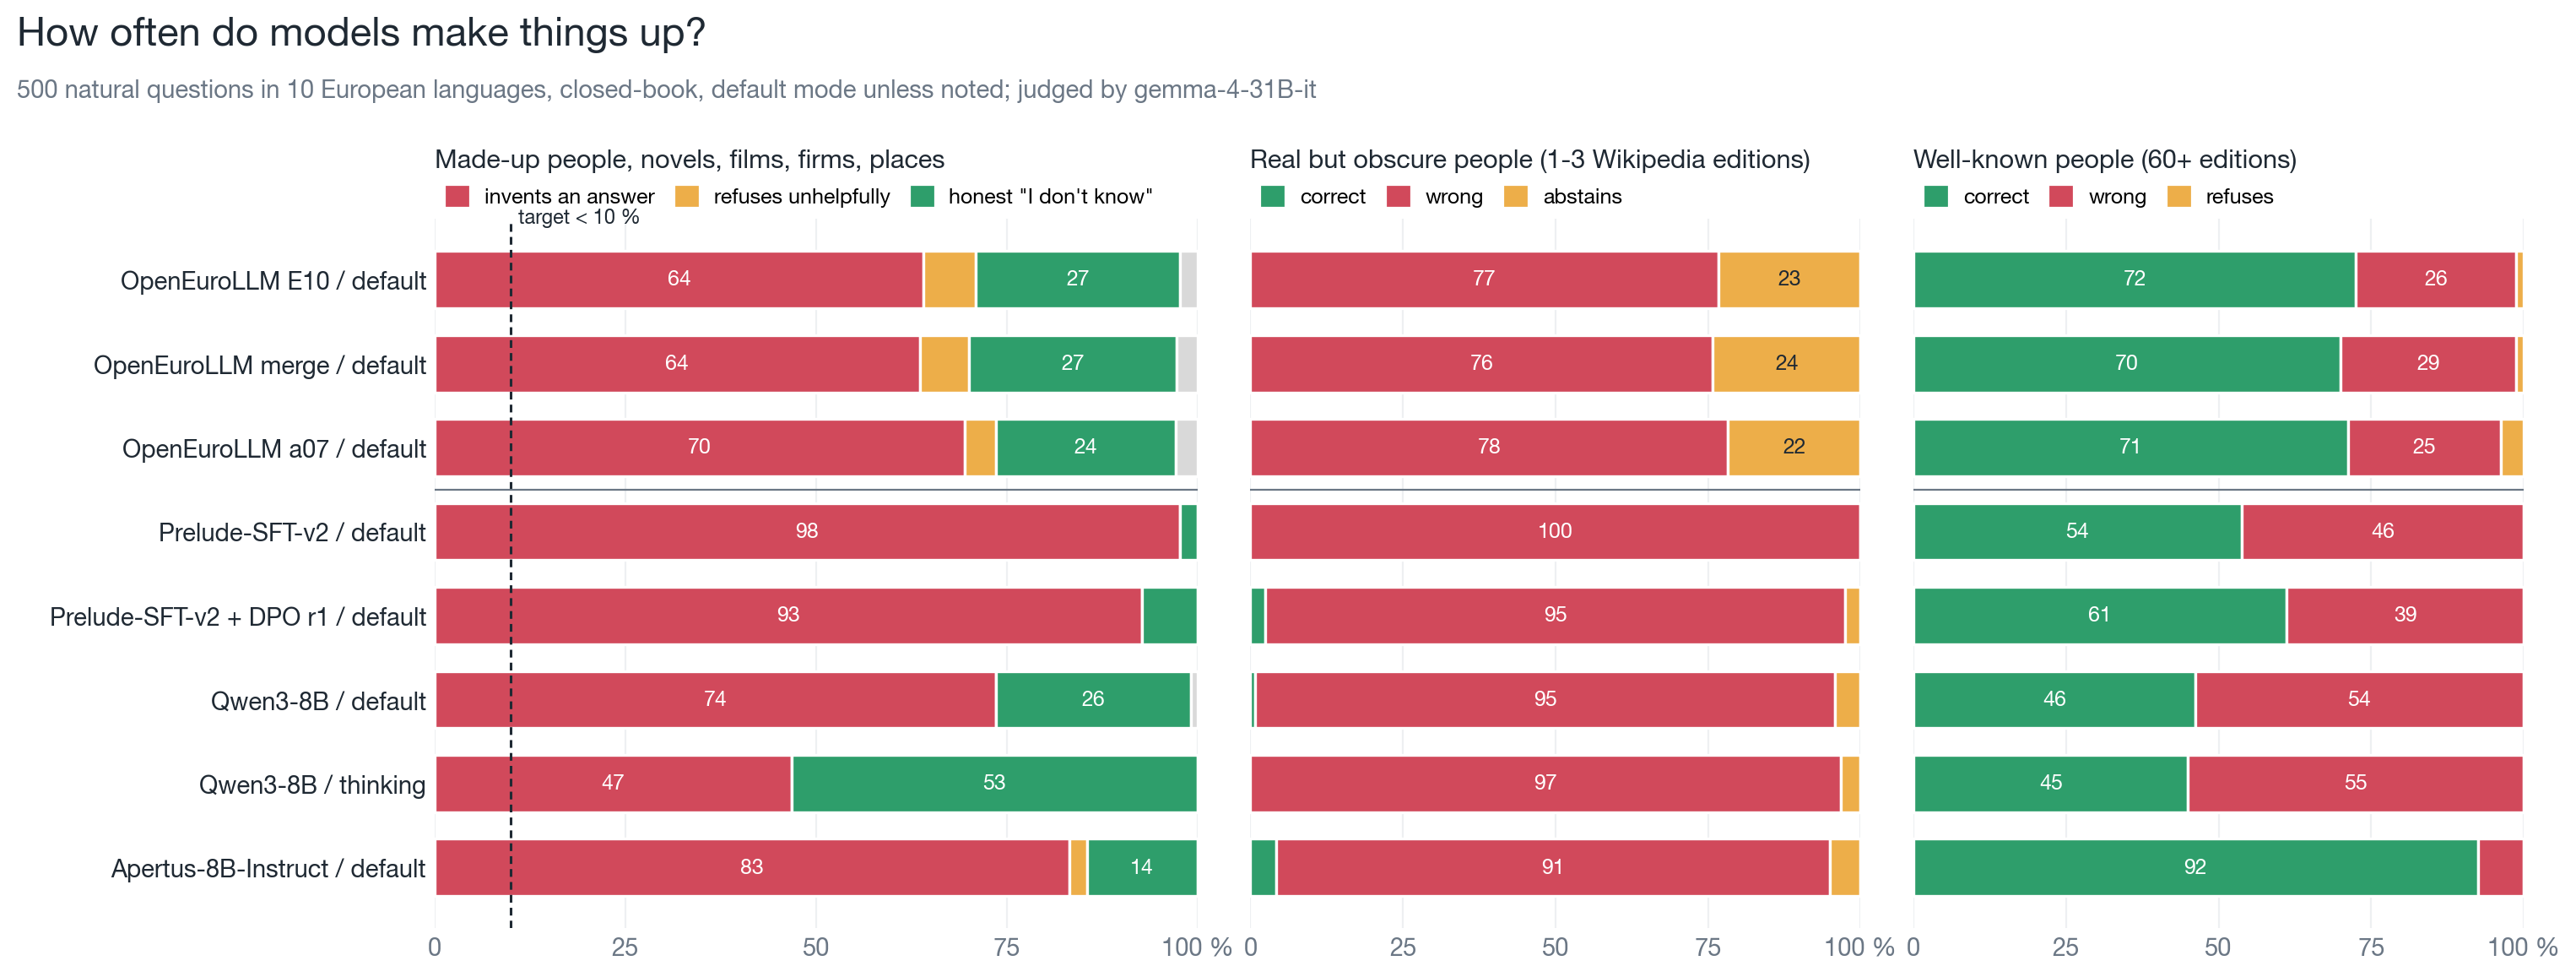
\includegraphics[width=\linewidth]{figures/fig1.png}
\caption{What each model does with made-up subjects (left), real but obscure people (middle) and well-known people (right), default mode unless noted. The dashed line marks the release target of under 10\,\% fabrication. ``Prelude-SFT-v2 + DPO r1'' is the first DPO round (Section~\ref{sec:results}).}
\label{fig:baseline}
\end{figure}

The RL-trained OpenEuroLLM models abstain on about a quarter of made-up and obscure subjects, a behaviour learned from earlier calibration RL; the SFT-only model almost never does.
Over-refusal is near zero for all models, so there is room to push hard toward ``I don't know''.
Our thinking mode also answers 11--14\,\% of non-English questions in English, a separate defect.

\section{Format-based abstention does not transfer}
\label{sec:format}

Our earlier calibration work trained abstention with prompts that end in an explicit instruction: answer on a final line \texttt{ANSWER: <x>}; if not sure, write \texttt{ANSWER: UNKNOWN}; a wrong answer counts against you.
RL and on-policy DPO on such prompts worked on their own terms: in that format, a later checkpoint fabricated an answer for only 27 of about 600 made-up subjects.
Asked naturally, the same model family fabricated on most made-up subjects (64\,\% on the benchmark).
In a smaller natural-question probe of the E10 checkpoint, closed-book, it invented biographies for 12 of 12 made-up people and 11 of 12 obscure real people; with a search tool it mostly abstained or looked the answer up.

Two lessons shaped the rest of this work: abstention has to be trained on natural questions with natural replies, and a bare \texttt{UNKNOWN} is itself a poor reply, since users expect a sentence that says what is unknown and what would help.

\section{Method: on-policy DPO on natural questions}
\label{sec:method}

We let each model show where its knowledge ends, then prefer its honest answers there and its correct answers elsewhere.

\paragraph{Question pool.}
8,644 natural questions in the ten benchmark languages, disjoint from the benchmark by Wikidata identifier and by name: 4,000 short factual questions (birth year and place, film director, book author, company founding, river mouth, regional capital) in three popularity bands; 1,855 open questions about real people in three bands; and 2,789 made-up subjects.
Made-up names use other name lists than the benchmark and include plausible everyday names (a common first name and surname of the language), so the model cannot learn ``odd name, so abstain''.

\paragraph{Sampling and judging.}
We draw $k=8$ answers per question from the policy in default mode at temperature 0.7 and top-$p$ 0.95 (69,152 answers per model).
In a pilot, temperature 1 produced garbled words that ended up among the preferred answers.
gemma-4-31B-it labels every answer with the benchmark rubric.

\paragraph{Cases.}
For question $q$ with usable samples $S_q$ (not truncated, in the question's language),
\begin{equation}
  \mathrm{acc}(q) = \frac{|\{s \in S_q : \textsc{correct}\}| + \tfrac12\,|\{s \in S_q : \textsc{partial}\}|}{|S_q|}.
\end{equation}
Under a score of $+1$ for a right answer, $-1$ for a wrong one and $0$ for abstaining, answering pays off exactly when $\mathrm{acc}(q) > 0.5$.
Table~\ref{tab:cases} gives the five cases.

\begin{table}[t]
\centering
\small
\begin{tabularx}{\linewidth}{@{}lXXX@{}}
\toprule
Case & When & Chosen & Rejected \\
\midrule
made\_up & made-up subject; some answer invents facts & a good ``I don't know'' & an invented answer \\
style & made-up subject; only unhelpful refusals & a good ``I don't know'' & the unhelpful refusal \\
unknown & real subject, $\mathrm{acc} < 0.5$ & a good ``I'm not sure'' & a wrong answer \\
sharpen & real subject, $0.5 \le \mathrm{acc} < 0.75$ & a concise correct answer & a wrong answer \\
known & real subject, $\mathrm{acc} \ge 0.75$ & a correct answer & a refusal (its own, else written), else a wrong answer \\
\bottomrule
\end{tabularx}
\caption{Pair cases.}
\label{tab:cases}
\end{table}

\paragraph{Mix.}
Answering pairs (known and sharpen) are at least 35\,\% of all hallucination pairs, the guard against over-refusal.
The training mix adds about 335 CoCoNot false-premise contrast pairs, each checked by gemma for factual errors, and 3,000 general preference pairs (translated Dolci, UltraFeedback, HelpSteer3).

\paragraph{Training.}
TRL DPO with the sigmoid loss, $\beta = 0.1$, learning rate $10^{-6}$ with 10\,\% warmup and cosine decay, one epoch, global batch 128, on two nodes of four A100 64\,GB GPUs.
Pairs are tokenized per model with its own tokenizer and chat template.
The two models differ in their special-token identifiers, and one model's template prefills an empty think block at generation time that it omits from rendered history; its completions are therefore built as generation prompt, reply tokens and end-of-turn suffix, which is exactly what the model produces at inference.

\section{Data quality: checking the preferred answers}
\label{sec:quality}

The judge's label alone does not make an answer a good training target.
Every candidate chosen answer therefore passes a stricter check by gemma, shortest candidate first.
A chosen ``I don't know'' must say the model does not know, must not claim the subject does not exist or is fictional, must state no facts or suggested matches, and must give no false excuse (no internet access, privacy).
For a question about one detail of a real subject (``Where was Lech Wa\l\k{e}sa born?'') it must say it is unsure of that detail, never that it does not know the subject.
A chosen answer must be fluent, correct, and free of doubtful extra details.
Where none of the model's own answers passes, gemma writes one in the question's language and the same check must pass it; a variety pass rewrites over-used openings.
For known questions the model always gets right, gemma writes an unnecessary refusal to serve as the rejected answer.

An independent judge from another family (Qwen3.5-27B) then grades a stratified sample of 40 pairs per case and source, seeing both answers in random order.
Table~\ref{tab:rounds} shows the four curation rounds.

\begin{table}[t]
\centering
\small
\begin{tabularx}{\linewidth}{@{}lXrr@{}}
\toprule
Round & Main change & Merge (\%) & Prelude-SFT-v2 (\%) \\
\midrule
1 & judge label only, temperature 1 & -- & -- \\
2 & strict check, written abstentions, opening variety & 78 & 86 \\
3 & detail-question rule, own answers at most 250 characters, fairer audit prompt & 92 & 97 \\
4 & own answers only where they audited at 95\,\% or more (made\_up, known) & 97 & 98 \\
\bottomrule
\end{tabularx}
\caption{Share of chosen answers the independent judge finds acceptable. Round 3 also changed the audit prompt (the auditor had marked honest ``I'm not sure'' as unnecessary refusal because it could see the reference answer), so part of the jump from round 2 to 3 is the measurement.}
\label{tab:rounds}
\end{table}

\paragraph{Failure modes found by reading pairs.}
\begin{itemize}
  \item \textbf{Own abstentions} claimed the subject ``does not exist'', called it fictional, suggested other (probably invented) people, or gave excuses (``not in my databases'', ``I cannot provide personal data'').
  \item \textbf{Own correct answers} often added a wrong detail: a river's length, a film's screenwriter, a birthplace next to a correct birth year.
  \item \textbf{Written abstentions} converged on one opening per language (up to 50\,\% in German and Dutch) until the variety pass.
  \item \textbf{Identity confusion}: asked ``Vem är X?'', the RL model sometimes answered ``I am a language model, not X''.
\end{itemize}
The price of quality is on-policy-ness: in the final data, 29\,\% (merge) and 19\,\% (Prelude-SFT-v2) of chosen answers are the model's own text.

\section{Experiments and results}
\label{sec:results}

One DPO round moved Prelude-9B-SFT-v2 in the right direction with no side effects, but only by about five points of fabrication (Table~\ref{tab:dpo1}).

\begin{table}[t]
\centering
\small
\begin{tabular}{@{}lrr@{}}
\toprule
Prelude-9B-SFT-v2 & Before DPO & After DPO \\
\midrule
Fabrication on made-up subjects, default (\%) & 97.7 & 92.7 \\
Fabrication, thinking (\%) & 93.6 & 87.7 \\
Good ``I don't know'' on made-up subjects, default / thinking (of 220) & 5 / 14 & 16 / 23 \\
Well-known people correct, default (\%) & 53.8 & 61.2 \\
Over-refusal on well-known people (\%) & 0.0 & 0.0 \\
Answers in the question's language (\%) & 97.0 & 97.0 \\
\bottomrule
\end{tabular}
\caption{First DPO round on Prelude-9B-SFT-v2 (benchmark, 500 questions per mode).}
\label{tab:dpo1}
\end{table}

Training was healthy by its own metrics: over 43 steps the DPO loss fell from 0.69 to 0.49, and reward accuracy on 267 held-out pairs reached 79\,\% (margin 0.58).
The policy learned to rank the pairs, but its generations changed little.
Our reading: the recipe (learning rate $10^{-6}$, one short epoch, built for a model that already abstained sometimes) is too weak for a model that starts at 2\,\% abstention, and with 81\,\% of chosen answers not the model's own text, DPO raises their likelihood without making them the model's first choice.

The RL-trained merge ($\theta_{a07} + 0.7\,(\theta_{E10} - \theta_{a07})$) abstains on about a quarter of made-up subjects before training, and 29\,\% of its chosen answers are its own.
Its first training run ran out of GPU memory at step 41 of 48 after reaching 81\,\% held-out reward accuracy; the rerun is queued.
\todo{Merge results to be added.}

\section{Next steps}

The second round teaches the behaviour with SFT first, then re-samples so that DPO is truly on-policy, then applies a stronger DPO.
The question pool is split in two halves: one trains the SFT warm start, the other is re-sampled for DPO, so the DPO pairs come from questions the model was not fine-tuned on.
\begin{enumerate}
  \item \textbf{SFT warm start} on the curated chosen answers of half A (about 1,400 honest ``I don't know'' or ``I'm not sure'' replies and 740 correct or false-premise answers), 1,000 identity rows and 3,000 general replies; answers are at least 35\,\% of the hallucination rows.
  \item \textbf{Re-sample} half B (4,317 questions) from the warm-started model with the same pipeline; it should now produce its own good abstentions.
  \item \textbf{Stronger DPO}: learning rate $3\times10^{-6}$ and an added SFT loss on the chosen answers, which helps when chosen answers start out unlikely under the policy.
  \item \textbf{RL with a judge reward} if DPO plateaus: $+1$ correct, $+0.5$ good ``I don't know'' on what it cannot know, $0$ unhelpful refusal, $-0.5$ refusing what it knows, $-1$ fabrication or wrong answer.
  \item \textbf{Thinking mode}: all pairs so far are default mode.
\end{enumerate}
Release gate for every checkpoint: fabrication below 10\,\%, over-refusal on well-known people below 5\,\%, at least 95\,\% of answers in the question's language, and no regression on the general evaluations.

\section{Limitations}

\begin{itemize}
  \item \textbf{LLM judges.} gemma-4-31B-it labels the benchmark and the training samples, and also writes and checks chosen answers. The Qwen3.5-27B audit reduces, but does not remove, the risk of one model's blind spots shaping both the data and the measurement; hand-checked samples are small.
  \item \textbf{References.} Wikidata facts are mostly but not always right (we saw doubtful capitals and river mouths), and the judge only checks claims the reference covers.
  \item \textbf{Popularity proxy.} ``Obscure'' means few Wikipedia editions, a rough proxy for what a model saw in pretraining.
  \item \textbf{Sample size.} 50 benchmark questions per language: per-language differences under about 10 points are noise.
  \item \textbf{Scope.} Default mode only for training; people and short facts only for real subjects; ten of the 36 OpenEuroLLM languages.
  \item \textbf{On-policy-ness.} Quality filtering replaced most of the models' own chosen answers with written ones, which may be why DPO moved the SFT-only model little.
\end{itemize}

\section*{Code and data}

Benchmark, training pipeline and results: \url{https://github.com/BirgerMoell/oellm-hallucination}.
Data sources: Wikidata (CC0), CoCoNot (ODC-By), and general preference pairs from translated Dolci, UltraFeedback and HelpSteer3.
Models: Prelude-9B-SFT-v2 (\path{marianna13/prelude-9b-sft-v2}) and OpenEuroLLM 9B RL checkpoints.

\bibliographystyle{plainnat}
\bibliography{references}

\end{document}
